\chapter{Estudio estratégico}
\textit{Los \textit{nonogramas} junto otros gigantes rompecabezas de <<papel y lápiz>> tales como: sudoku, crucigramas, hundir la flota, ahorcado... se han adaptado a
una era en la que está gobernada por las nuevas plataformas tecnológicas. Y más concretamente, en estos tiempos de incertidumbre, confinamientos e incluso ocio han propiciado que estos
puzzles se hagan cada más presentes en nuestras vidas, alejándose una posible obsolescencia.}

\section{Nonogramas en la era Digital}

Pese a que la era Digital ofrece un amplio abanico de medios o plataformas que han incluido y popularizado estos rompecabezas, en
este apartado nos enfocaremos en el de las aplicaciones móviles.

Para que el estudio sea exhaustivo, se explorarán aquellas aplicaciones disponibles en las principales tiendas de aplicaciones para 
las plataformas \textit{Android} e \textit{iOS}, \textit{Google Play} y \textit{App Store} respectivamente.

\subsection{Nonograms Katana}
Nonograms Katana es una aplicación con una remarcada temática nipona, que permite al usuario resolver una gran variedad de \textit{nonogramas},
de una gran variedad de categorías y dimensiones, como se puede comprobar en la Figura~\ref{fig:katana2-1}.

\begin{figure}[H]
   \centering
   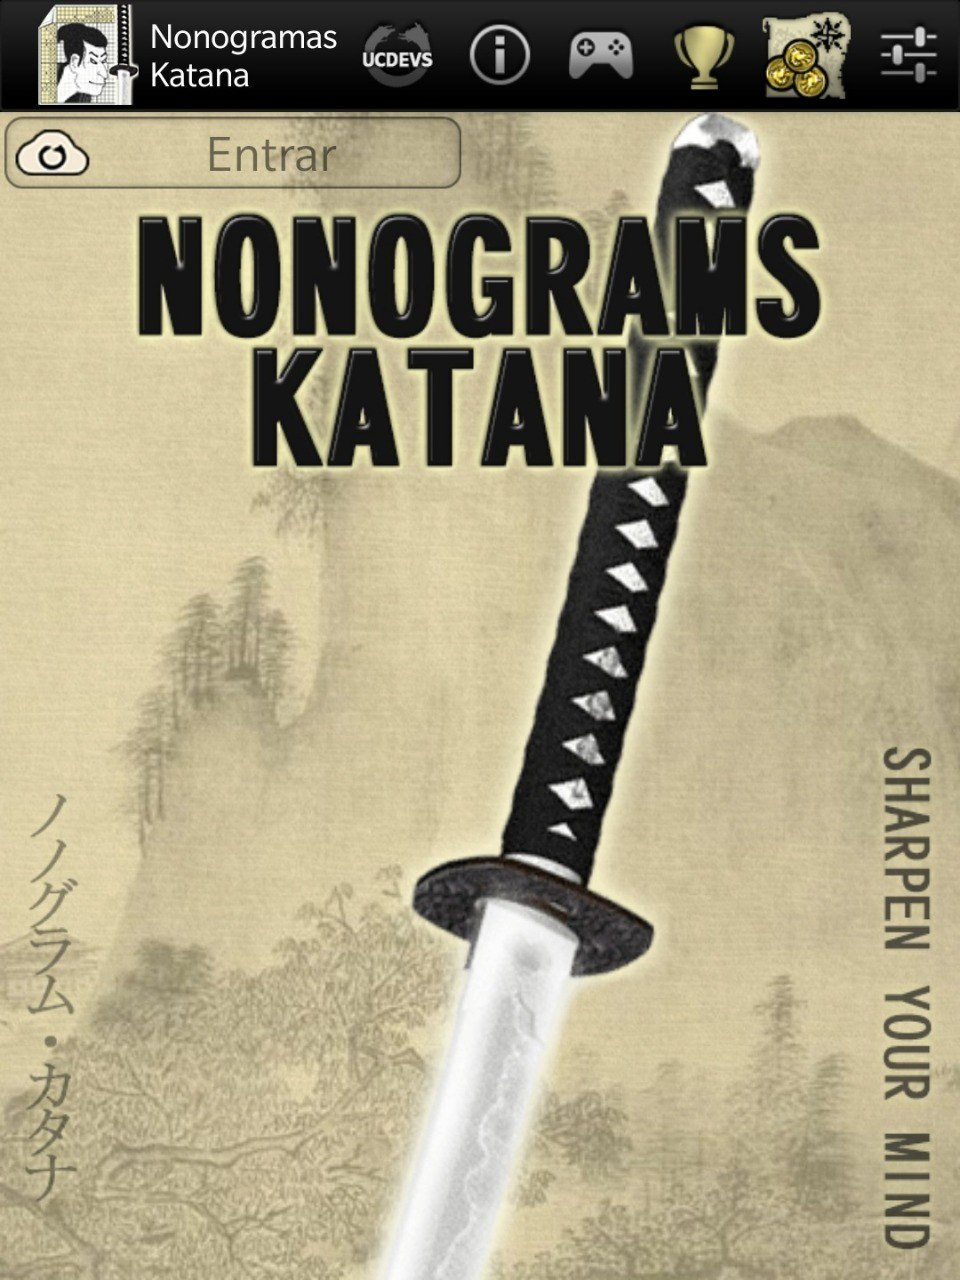
\includegraphics[scale=.15]{images/nonokatana1.jpg}
   \caption{Pantalla principala de Nonograms Katana}
   \label{fig:katana1}
 \end{figure}

 Además, como se puede apreciar en la Figura~\ref{fig:katana2-2}, se incluye la resolución de \textit{nonogramas} a color, en el que mediante un selector
 de colores el usuario pinta cada una de las celdas, resolviendo de este modo el \textit{nonograma}.

 \begin{figure}[H]
   \centering
   \begin{subfigure}[b]{0.47\linewidth}
     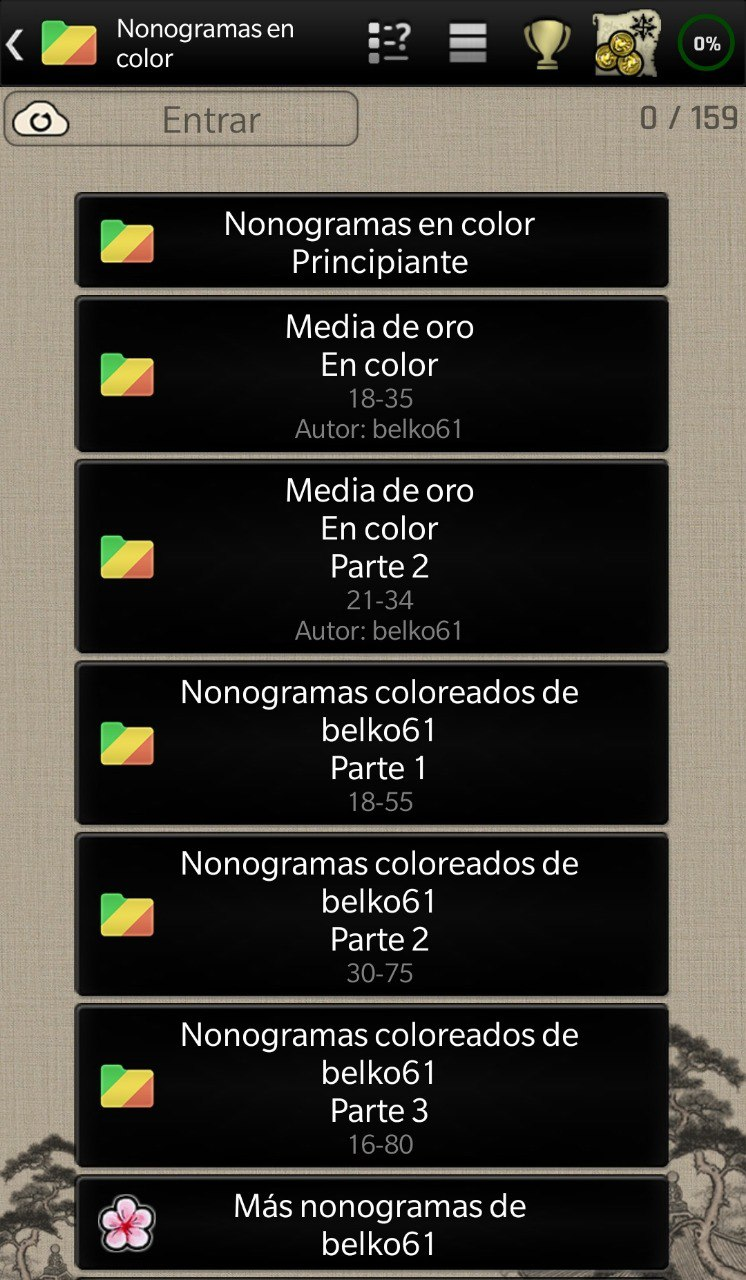
\includegraphics[width=\linewidth]{images/nonokatana2.jpg}
     \caption{Selector de niveles Nonogramas a color}
     \label{fig:katana2-1}
   \end{subfigure}
   \begin{subfigure}[b]{0.47\linewidth}
     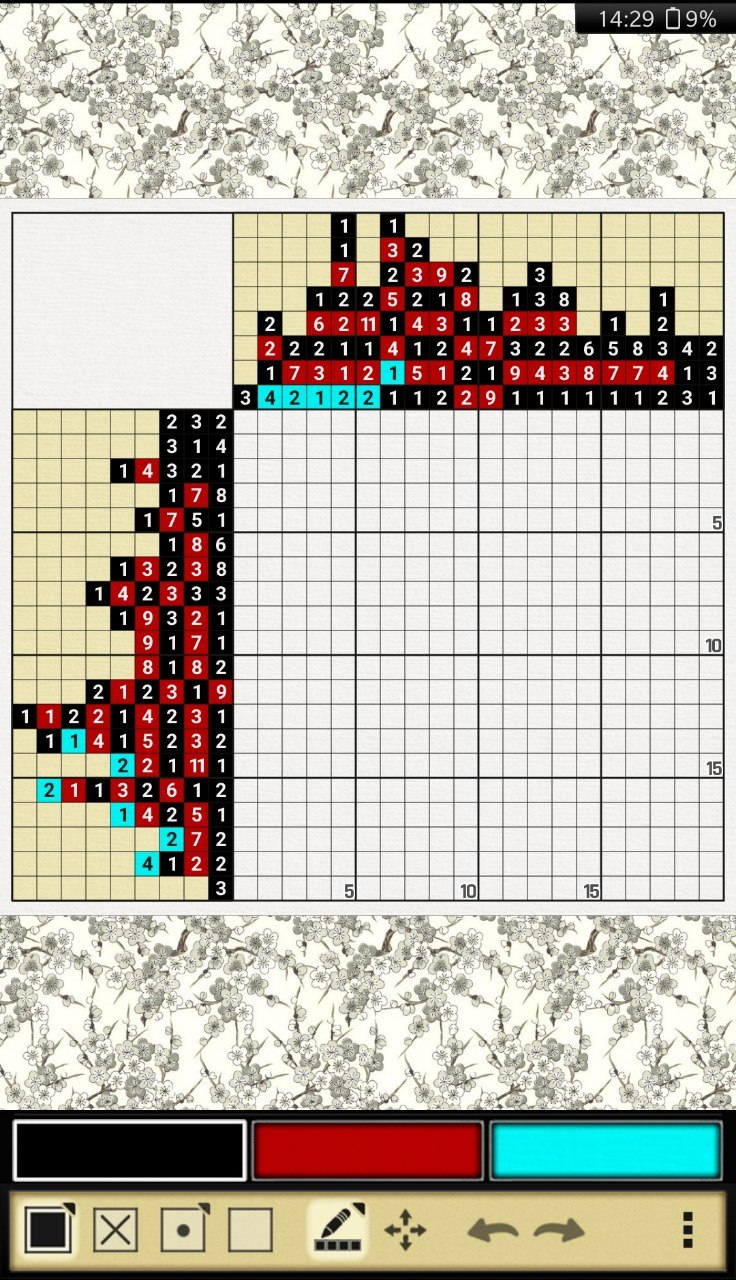
\includegraphics[width=\linewidth]{images/nonokatana3.jpg}
     \caption{Pantalla de resolución de un nivel 20x20 a color}
     \label{fig:katana2-2}
   \end{subfigure}
   \caption{Pantallas de Nonograms Katana con modalidad a color.}
   \label{fig:katana2}
 \end{figure}
 
 El aplicativo sigue la corriente clásica y no permite al usuario resolver los \textit{nonogramas} bajo un número determinado de \textit{vidas} 
 o intentos \textit{(disminuyendo su valor al pulsar sobre celdas erróneas)}, siendo algo tediosa la experiencia de juego, ya que puede acarrear fallos
 durante su resolución.

 Una característica notable de la aplicación es la de permitir al usuario crear sus propios \textit{nonogramas}, compartirlos con la comunidad, y resolver los de
 otros usuarios. Sin embargo, está propiedad no es su principal función y aparece bloqueda si no estás registrado, además de estar limitada por restricciones como los de la 
 Figura~\ref{fig:katana3}.

 El aplicativo presenta la propiedad de multilenguaje, no obstante, este presenta errores en sus traducciones, como se puede comprobar en la figura anteriormente
 citada.

 \begin{figure}[H]
   \centering
   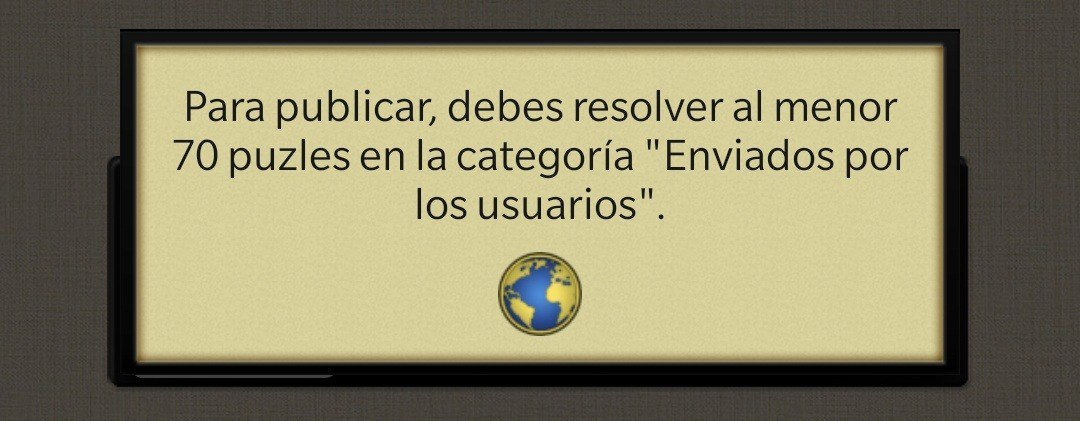
\includegraphics[scale=.175]{images/nonokatana4.jpg}
   \caption{Modal de restricción en publicación en Nonograms Katana}
   \label{fig:katana3}
 \end{figure}
 

\subsection{Nonogram.com - Picture cross number puzzle}

Una de las aplicaciones más descargadas dentro de la categoría puzzle con más de diez millones de descargas en la tienda \textit{Google Play}, 
presenta una interfaz amigable y limpia.

Hace un buen uso de animaciones, destacando la experiencia de juego, algunas bastante remarcables como cuando la que se muestra en la 
Figura~\ref{fig:picture1-2}, en cuanto finalizas un nivel.

\begin{figure}[h!]
   \centering
   \begin{subfigure}[b]{0.45\linewidth}
     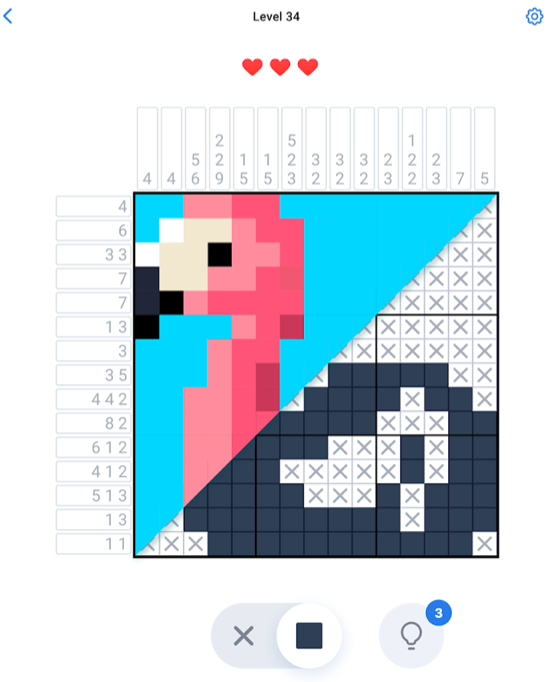
\includegraphics[width=\linewidth]{images/picturecross1.png}
     \caption{Pantalla de resolución de un nivel 15x15}
     \label{fig:picture1-1}
   \end{subfigure}
   \begin{subfigure}[b]{0.45\linewidth}
     
\includegraphics[width=\linewidth]{images/picturecross2.png}
     \caption{Pantalla de felicitación al resolver el nivel}
     \label{fig:picture1-2}
   \end{subfigure}
   \caption{Pantallas de Nonogram.com}
   \label{fig:picture1}
 \end{figure}

Como característica extra de juego, como se visualiza en la Figura~\ref{fig:picture1-1}, la barra inferior de juego incorpora un botón llamado \textit{Pista}, 
con el que después de ser seleccionado, 
el usuario puede clicar sobre una celda determinada y descubrir si es correcta sin restar una vida, teniendo limitada esta opción a tres usos por nivel.

\begin{figure}[H]
   \centering
   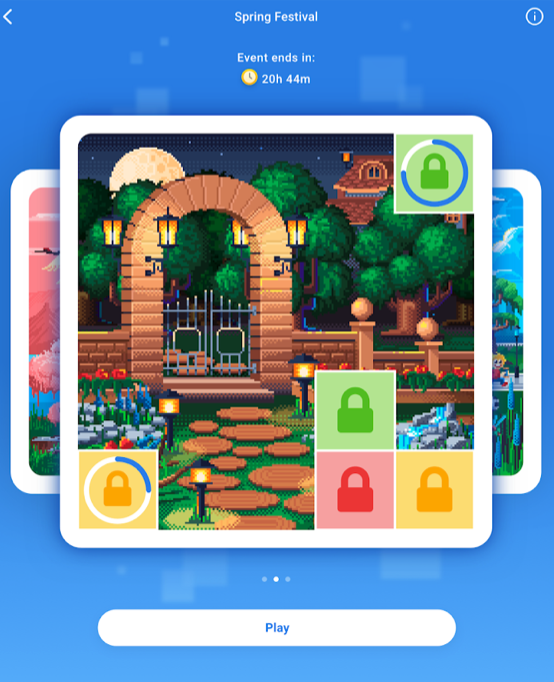
\includegraphics[scale=.25]{images/picturecross3.png}
   \caption{Pantalla de Evento Primavera de Nonogram.com}
   \label{fig:picture2}
 \end{figure}

En el aplicativo, de forma recurrente, aparecen \textit{Eventos} en los que el usuario puede resolver un conjunto de \textit{nonogramas} especiales relacionados
con una temática concreta, representada en la Figura~\ref{fig:picture2}.
 
La solución, como se ha podido comprobar, es de las más completas de las disponibles, no obstante, incluye publicidad excesivamente intrusiva para el usuario,
presente en casi todas sus funcionalidades, que entorpecen la experiencia de juego, incluso llegando a entorpecer al jugador.

\subsection{Nono Infinite}
Este producto destaca por su interfaz \textit{arcade}, con una clara intención de ser dirigida para todos los públicos, constrantando colores muy vivos,
con formas que recuerdan mucho a juegos clásicos para niños, se puede ver reflejado en las Figuras~\ref{fig:infinite1}.

\begin{figure}[h!]
   \centering
   \begin{subfigure}[b]{0.49\linewidth}
     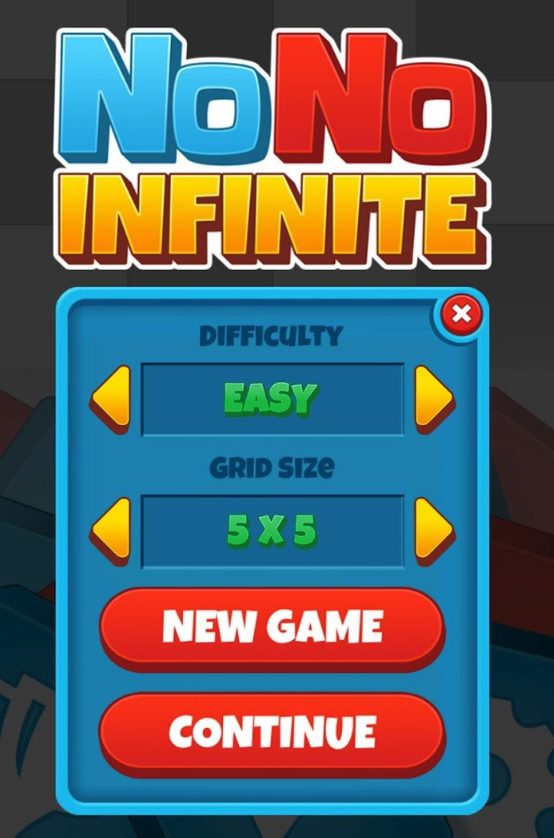
\includegraphics[width=\linewidth]{images/infinite1.png}
     \caption{Pantalla selector de nivel}
     \label{fig:infinite1-1}
   \end{subfigure}
   \begin{subfigure}[b]{0.49\linewidth}
     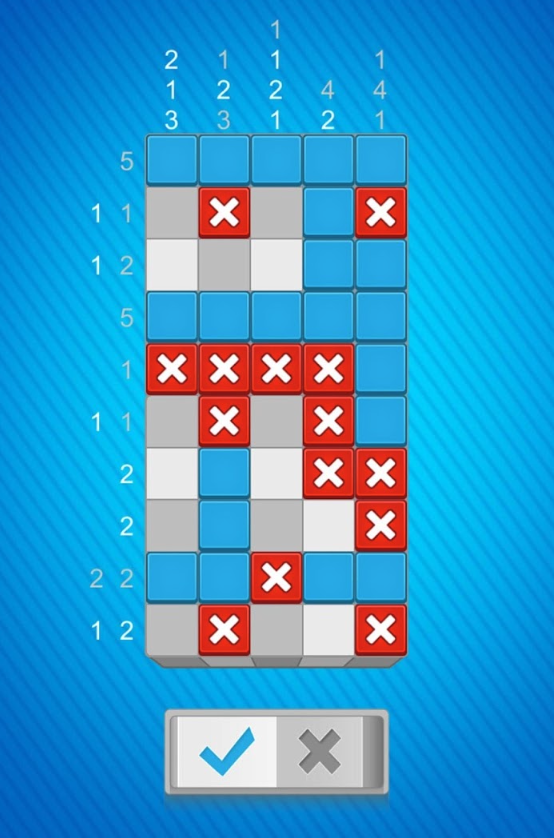
\includegraphics[width=\linewidth]{images/infinite2.png}
     \caption{Pantalla de resolución de un nivel 5x10}
     \label{fig:infinite1-2}
   \end{subfigure}
   \caption{Pantallas de selección de nivel y juego de Nono Infinite}
   \label{fig:infinite1}
 \end{figure}

Como peculiaridad, presenta \textit{nonogramas} de dimensiones poco usuales que difieren mucho de los clásicos, como el 5x10 presente en la
Figura~\ref{fig:infinite1-2}. Así mismo, permite cambiar la dificultad de los niveles manteniendo las dimensiones del mismo, sin embargo,
esta puede parecer un poco "\textit{artificial"} ya que únicamente aumenta las distancias de las celdas correctas.

Resulta interesante cómo la solución aprovecha el apartado del tutorial, para habituar al usuario de forma interactiva con las reglas clásicas de los 
\textit{nonogramas}, controles del mismo y consejos más avanzados, sobretodo para niveles más complejos, Figura~\ref{fig:infinite2}.

\begin{figure}[H]
   \centering
   \begin{subfigure}[b]{0.4\linewidth}
     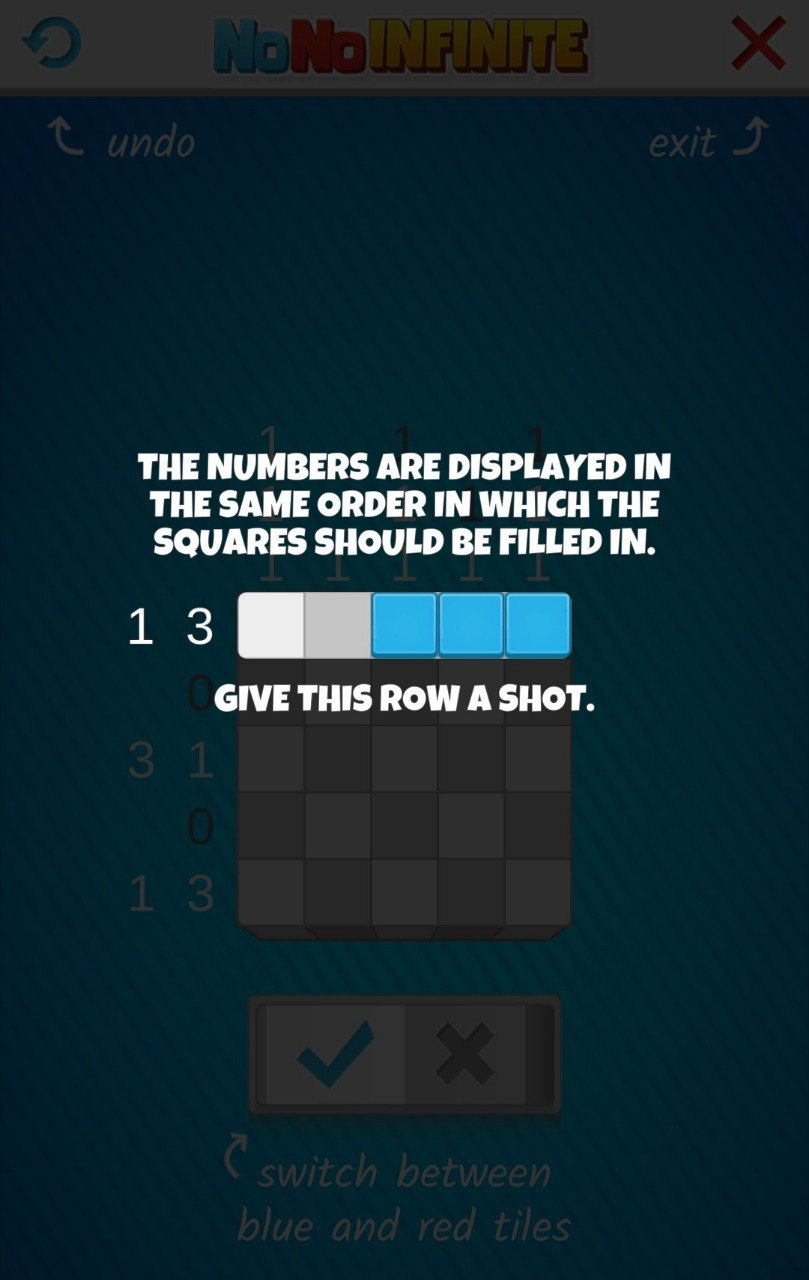
\includegraphics[width=\linewidth]{images/infinite3.jpg}
   \end{subfigure}
   \begin{subfigure}[b]{0.4\linewidth}
     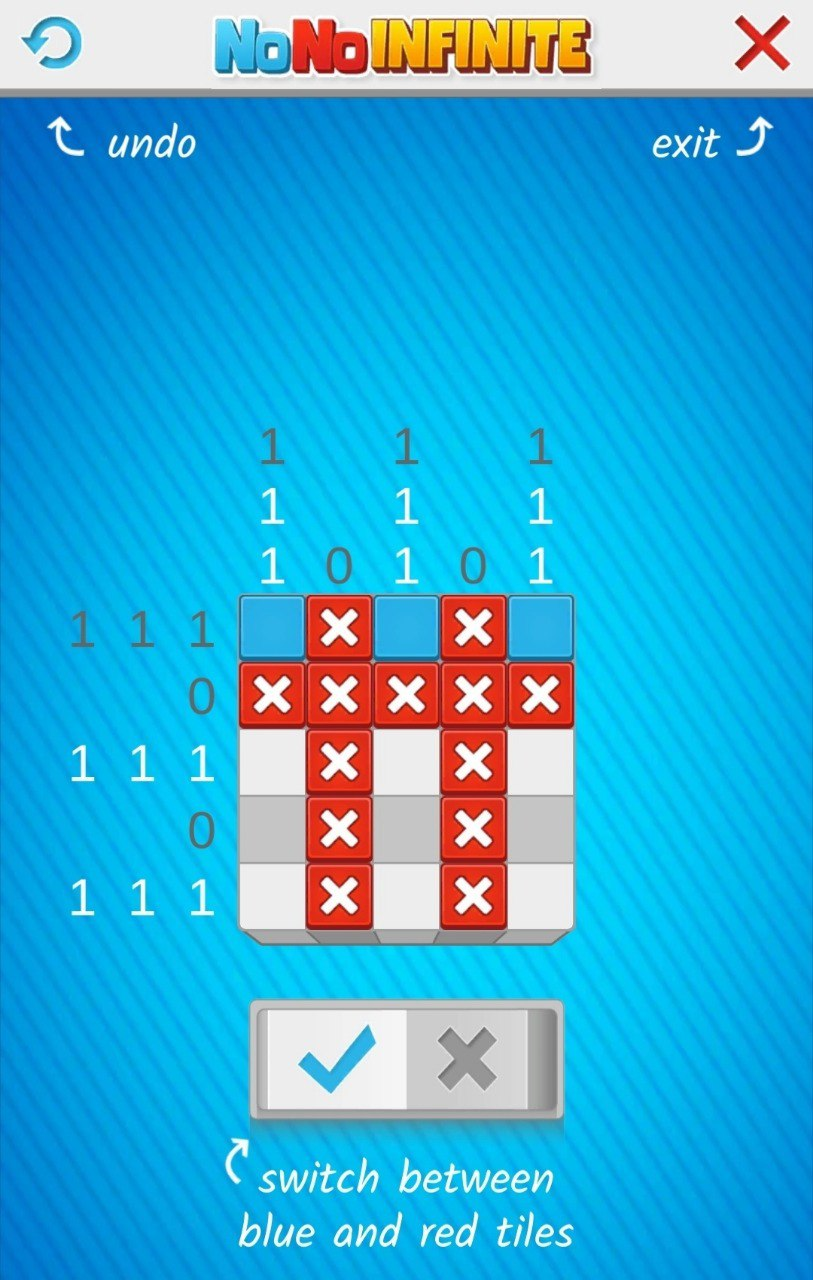
\includegraphics[width=\linewidth]{images/infinite4.jpg}
   \end{subfigure}
   \caption{Pantallas de tutorial en Nono Infinite}
   \label{fig:infinite2}
 \end{figure}

 \subsection{Family Crest Nonogram}

 Family Crest Nonogram es un juego que, pese a que no destaque por su apartado gráfico e interfaz de usuario, presenta muchas características que lo diferencian
 del resto de soluciones del género.

 Lo más remarcable de la aplicación es que tenga establecido su uso en modo \textit{landscape} (apaisado), adaptándose al formato de la mayoría de géneros
 de juegos de móvil. Sin embargo, este puede ser un punto negativo para muchos, ya que priva al jugador la esencia de estar jugando a un pasatiempo,
 recordándo más a la de un \textit{videojuego}.

 \begin{figure}[h!]
  \centering
  \begin{subfigure}[b]{0.49\linewidth}
    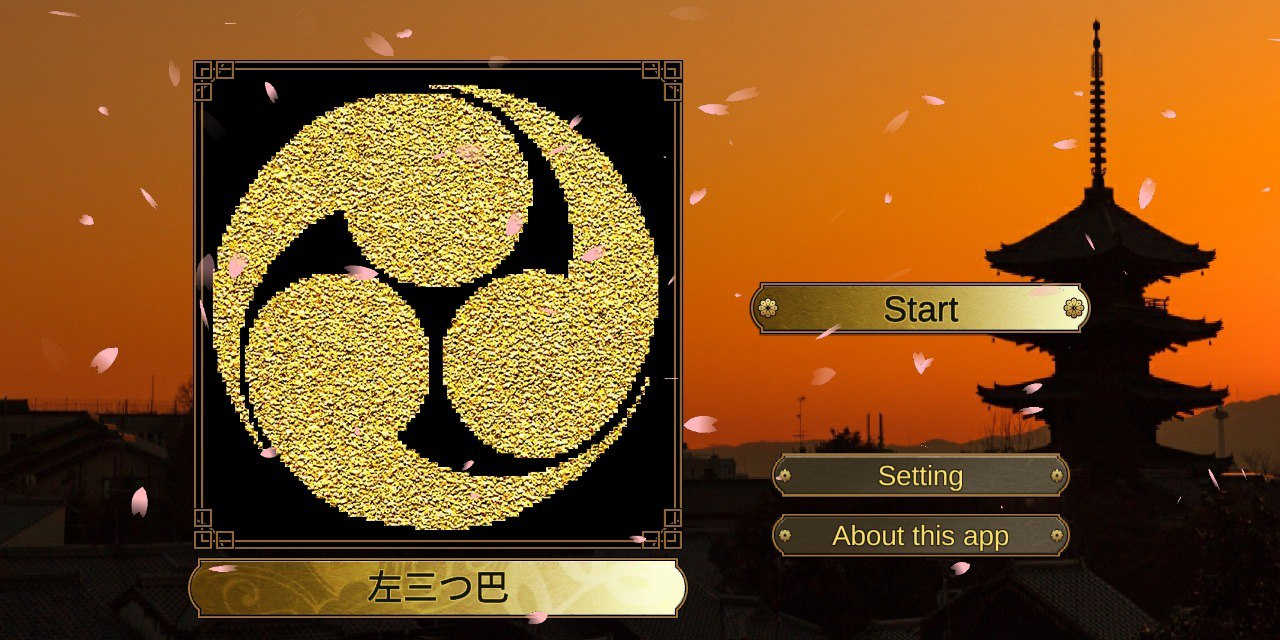
\includegraphics[width=\linewidth]{images/familycrest1.jpg}
    \caption{Pantalla principal}
    \label{fig:family1-1}
  \end{subfigure}
  \begin{subfigure}[b]{0.49\linewidth}
    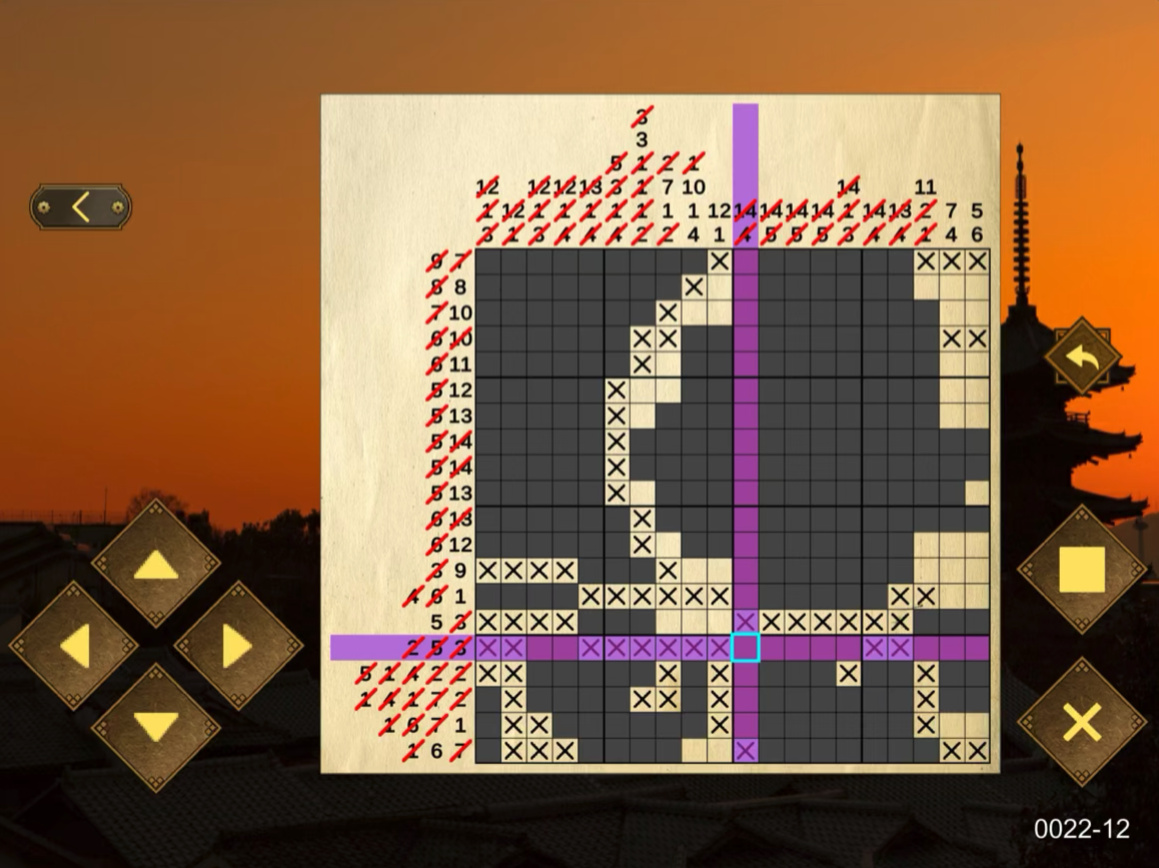
\includegraphics[width=\linewidth]{images/familycrest2.png}
    \caption{Pantalla de resolución de un nivel 20x20}
    \label{fig:family1-2}
  \end{subfigure}
  \caption{Pantallas de Family Crest}
  \label{fig:family1}
\end{figure}

No obstante, su experiencia de juego es muy notable, ya que presenta una \textit{cruceta} (para moverse por cada una de las celdas) 
y botones físicos de acción que facilitan un mayor control,
Figura~\ref{fig:family1-2}, además de incorporar una música ambiente que acompaña al usuario cada vez que  está jugando un nivel.

\section{Ánalisis de las aplicaciones}

Al analizar las aplicaciones enfocadas al submundo de los \textit{nonogramas}, vemos que siguen un patrón de similitudes, que resultan sustanciales 
para el desarrollo de una solución del género rompecabezas, además de ciertas peculiaridades que parecen interesantes para su inclusión en la solución.
Es importante también remarcar y apartar aquellas características que puedan ser perjudiciales para una primera versión de la solución.
A continuación, se muestra un tabla representativa de cada una de las características estudiadas, donde se objetarán su final inclusión en el aplicativo:

\renewcommand\theadalign{b}
\renewcommand\theadfont{\bfseries}
\renewcommand\theadgape{\Gape[1pt]}
\renewcommand\cellgape{\Gape[1pt]}
\newcommand{\cmark}{{\ding{51}}}
\newcommand{\xmark}{{\ding{55}}}
\begin{table}[H]
  \caption{Comparativa de características entre aplicaciones de interés y su inclusión como requisito}
    \begin{tabular}{ | c | c | c | c | c | c |}
      \hline
      \thead{Característica \\ encontrada} & \thead{Nonogram \\ Katana} & \thead{Nonograma.com \\ Picture cross} & \thead{Nono \\ Infinite} & \thead{Family \\ Crest} & \thead{Incluido como \\ requisito} \\
      \hline
      \makecell{Aplicación \\ multiplataforma} &  \cmark  & \cmark  & \xmark & \cmark & \cmark \\
      \hline
      \makecell{Temática \\ especial} &  \cmark  & \xmark  & \cmark & \cmark & \cmark \\
      \hline
      \makecell{Creación \\ nonogramas} &  \cmark*  & \xmark  & \xmark & \xmark & \cmark \\
      \hline
      \makecell{Opción de \\ autoguardado} &  \cmark  & \cmark  & \xmark & \xmark & \cmark* \\
      \hline
      \makecell{Registro de \\ usuario} &  \cmark  & \xmark  & \xmark & \xmark & \xmark \\
      \hline
      \makecell{Sincronización \\de niveles en nube} &  \cmark  & \xmark  & \xmark & \xmark & \cmark \\
      \hline
      \makecell{Juego \\ con \textit{vidas}} &  \xmark  & \cmark  & \xmark & \xmark & \cmark* \\
      \hline
      \makecell{Música \\ ambiente} &  \xmark  & \xmark  & \xmark & \cmark & \xmark \\
      \hline
      \makecell{Botón de \\ pistas} &  \xmark  & \cmark  & \xmark & \xmark & \xmark \\
      \hline
      \makecell{Botones físicos \\ de acción} &  \cmark  & \cmark  & \cmark & \cmark & \xmark \\
      \hline
      \makecell{Variedad de\\ visuales} &  \cmark  & \xmark  & \xmark & \xmark & \cmark \\
      \hline
      \makecell{Multi- \\ idioma} &  \cmark*  & \cmark  & \xmark & \xmark & \cmark \\
      \hline
      \makecell{Eventos \\ especiales} &  \xmark  & \cmark  & \xmark & \xmark & \xmark \\
      \hline
      \makecell{Nonogramas \\ a color} &  \cmark  & \xmark  & \xmark & \xmark & \xmark \\
      \hline
      \makecell{Tutorial \\ de juego} &  \cmark  & \cmark  & \cmark & \xmark & \cmark \\
      \hline
      \makecell{Sección \\ Leaderboard} &  \cmark  & \cmark  & \xmark & \xmark & \xmark \\
      \hline
      \makecell{Selector de \\ niveles} &  \cmark  & \xmark  & \xmark & \cmark & \cmark \\
      \hline
    \end{tabular}
    \label{fig:table1}
\end{table}

La inclusión de las características de la Tabla~\ref{fig:table1} se ven indicadas mediante la siguiente simbología:

\begin{enumerate}
	\item \cmark : Característica incluida en el aplicativo.
	\item \xmark : Característica no incluida en el aplicativo.
	\item \cmark* : Característica incluida en el aplicativo con ciertos matices.
\end{enumerate}

\section{Propuesta}
Visualizando las características reflejadas en la Tabla~\ref{fig:table1} sacamos la siguientes conclusiones de cara a la creación de la primera
versión de la aplicación como producto:

\begin{itemize}
  \item[$\bullet$] Ya que la mayoría de apps estudiadas son multiplataforma, el aplicativo funcionará para ambas plataformas \textit{Android} e \textit{iOS}.
  \item[$\bullet$] Seguirá una temática especial con el fin de diferenciarlas del resto, además de ir alternando entre temas diversos cambiando
  la interfaz de usuario.
  \item[$\bullet$] Tanto la resolución como la creación de los nonogramas será una de las funciones de la solución, sin ningún tipo de restricción.
  \item[$\bullet$] El usuario podrá usar \textit{servicios in-cloud} como: sincronización en nube o acceso a la base de datos sin tener que registrarse.
  \item[$\bullet$] La aplicación tendrá posibilidad multi-idioma, teniendo disponible inglés y español para esta primera versión, sin ningún tipo de errata.
  \item[$\bullet$] Se podrán jugar niveles de \textit{nonogramas} de diferentes dimensiones clásicas, recordando a los de los medios físicos tradicionales,
  previamente explicado su uso por un tutorial intuitivo. 
  \item[$\bullet$] Durante la resolución del nonograma, el usuario podrá resolverlo con una interfaz minimalista, en ausencia de botones físicos,
  además de poder alternar entre resolución con y sin \textit{vidas}.
  \item[$\bullet$] Muchas de las características estudiadas se han tomado como no esenciales y quedarán descartadas para la primera versión.
\end{itemize}